\todo[inline]{taskbench and hyperloom related work benchmarks}

After performing the task scheduling experiments using \estee{}, our next goal was to
find out how do other aspects of task runtimes (other than the scheduler) affect makespans of task
graph executions, and also to validate some of the rather surprising results of our experiments,
for example the competitiveness of the random scheduler, in a non-simulated setting. To do that, we
had to move from a simulator to a task runtime that can execute task graphs on an actual
distributed cluster.

We have decided to use \dask{}~\cite{dask} for our experiments, for
several reasons:
\begin{itemize}
	\setlength\itemsep{0.1em}
	\item It is very popular within the scientific community~\cite{dask-user-survey}, therefore any insights on
	      how it could be improved could benefit a wide range of users.
	\item It is implemented in Python, which makes it relatively easy to modify.
	\item It is quite versatile, because it allows executing arbitrary task graphs with dependencies and data
	      objects, and completely supports the task programming model described in
	      Chapter~\ref{ch:taskgraphs}.
	\item It uses a fairly standard distributed architecture with a centralized server that creates task
	      schedules and assigns tasks to a set of distributed workers. This maps well to the cluster
	      architecture used by \estee{}, and also to HPC clusters in general.
\end{itemize}

In terms of task scheduling, \dask{} uses a work-stealing scheduler, which has been
tuned extensively to support various use-cases and task graphs. Yet it is unclear whether
additional effort should be directed into improving the scheduler, or if there is another
bottleneck which should be prioritized.

To answer that question, we have analyzed the runtime performance and the bottlenecks of
\dask{} in \emph{Runtime vs Scheduler: Analyzing Dask's Overheads}\footnote{Note that this line of research follows after the task scheduler analysis described previously in
Chapter~\ref{ch:estee}, even though it was published at an earlier date.}~\cite{rsds}.
This work provides the following contributions:
\begin{enumerate}
	\item We have created a set of benchmarks containing diverse task graphs implemented in
	      \dask{}. This benchmark set was then used to analyze \dask{}'s
	      performance in various HPC-inspired scenarios. We have evaluated the per-task-overhead and
	      scalability of \dask{} and compared how different task scheduling algorithms affect
	      its performance.
	\item We demonstrate that even a naïve (completely random) scheduling algorithm can be in many common
	      situations competitive with the sophisticated hand-tuned work-stealing scheduler used in
	      \dask{}.
	\item We provide \rsds{}, an alternative \dask{} server that is
	      backwards-compatible with existing \dask{} programs and provides significant
	      speed-up vs the baseline \dask{} server in many scenarios, despite using a simpler
	      task scheduler implementation.
\end{enumerate}

Various descriptions of task graph benchmarks, \dask{} and \rsds{}
used in this chapter were adapted from our publication~\cite{rsds}.

\workshare{I have collaborated on this work with Ada Böhm, we have both contributed to it equally. Source code contribution statistics for
\rsds{} can be found on GitHub\footnoteurl{https://github.com/it4innovations/rsds/graphs/contributors}.}

\section{Dask}
\label{sec:rsds-dask}
% TODO: place Dask into SOTA and describe it more, if not already done in the SOTA chapter
\dask{} is a distributed task runtime implemented in Python that can parallelize
and distribute Python programs. It offers various programming interfaces (APIs) that mimic the
interfaces of popular Python packages. For example, \emph{Dask DataFrame} copies the
\texttt{pandas}\footnoteurl{https://pandas.pydata.org} interface for table processing and database
operations, \emph{Dask Arrays} copies the \texttt{numpy}\footnoteurl{https://numpy.org}
interface for tensor computations and \emph{Dask ML} copies the
\texttt{scikit-learn}\footnoteurl{https://scikit-learn.org} interface for machine learning. Thanks to this
interface compatibility, existing Python programs leveraging these libraries can often be
parallelized with \dask{} by changing only a handful of lines of code.

This is demonstrated in Figures~\ref{lst:dask-array-example} and~\ref{lst:dask-dataframe-example}, which show two
small Python programs that leverage the \emph{Dask Arrays} (Figure~\ref{lst:dask-array-example}) and \emph{Dask DataFrame}
(Figure~\ref{lst:dask-dataframe-example}) API.
Notably, the only difference between these programs (which are leveraging \dask{},
and thus can be parallelized), and a standard sequential version, is the change of imports from
\texttt{numpy} and \texttt{pandas} to \dask{} Python modules.

\begin{listing}[h]
	\caption{Example of a Python program that leverages the \dask{} Array API}
	\label{lst:dask-array-example}
	\begin{minted}[fontsize=\small]{python}
# import numpy as np
import dask.array as np

x = np.random.random((10000, 10000))
y = (y * 2 + x.T).mean(axis=1)
	\end{minted}
\end{listing}

\begin{listing}[h]
	\caption{Example of a Python program that leverages the \dask{} DataFrame API}
	\label{lst:dask-dataframe-example}
	\begin{minted}[fontsize=\small]{python}
# import pandas as pd
import dask.dataframe as pd

df = pd.read_csv("data.csv")

df2 = df[df.y > 0]
df3 = df2.groupby("name").x.std()
	\end{minted}
\end{listing}

\subsection*{Computational model}
\dask{} automatically transforms Python code leveraging these APIs into a task
graph, which is then executed in parallel, possibly on multiple nodes of a distributed cluster.
This enables almost transparent parallelization of sequentially looking Python code. However, apart
from these high-level interfaces, it is also possible to build a task graph manually, using the
\emph{Futures} interface, to define complex computational workflows.

The core computational abstraction of \dask{} is a \emph{task graph}, which
corresponds closely to the definition of task graphs in Chapter~\ref{ch:taskgraphs}. Each task
represents a single invocation of a Python function. The return value of the function forms its
\emph{output} (a data object), and the arguments of the function invocation define the
\emph{inputs} of the task.

One important aspect of the mapping between Python code and task graphs in \dask{}
is the concept of \emph{partitions}. It is a configuration parameter that essentially controls
the granularity of tasks created by \dask{} out of Python code that uses its APIs.
For example, a single line of Python code that performs a query over a \texttt{pandas}-like
table (also called DataFrame) will be eventually converted to a set of individual tasks that e.g.\
perform the query on a subset of the table's rows. The selected number of these tasks (or
partitions) is crucial, since it determines how effectively will the operation be parallelized. Too
few (large) tasks can cause computational resources to be under-utilized, while too many (small)
tasks can overwhelm the \dask{} runtime.

\subsection*{Architecture}
\dask{} supports multiple computational backends that can execute the task graphs
generated from Python code. The default backend is able to execute the task graph in a parallelized
fashion on a local computer, but there is also a distributed backend called
\emph{Dask/distributed}\footnoteurl{https://distributed.dask.org}
(or simply \emph{distributed}), which is able to execute task graphs on multiple
nodes. Since this backend is most relevant for task graph execution on distributed and HPC
clusters, our experiments focus solely on this backend, and any further reference to
\dask{} in this text will assume that it uses the \emph{distributed} backend.

In terms of architecture, \emph{distributed} is composed of three main components: the
\emph{client}, the \emph{server} and the \emph{worker}. A single
server and an arbitrary number of workers deployed together (e.g.\ on a local machine or a
distributed system) form a \dask{} cluster.

The \emph{client} is a user-facing library that offers various APIs used to define
computations in Python that can be converted into a task graph. Once the user defines the
computation, the client can connect to the \dask{} cluster (more specifically, to
the server), submit the task graph, wait for it to be computed and then gather the results. The
client can build the whole task graph eagerly on the user's machine and then send it to the server
for processing, however this can consume a lot of memory and network bandwidth if the task graph is
large. For certain types of task graphs, clients are able to send a much smaller, compressed
abstract representation of the task graph, which is only expanded on the server lazily, which can
help reduce memory and network transfer bottlenecks.

The \emph{server} is the central component of the cluster, which communicates with the
workers and clients through a network (usually TCP/IP) connection, handles client requests,
coordinates task execution on workers and manages the whole \dask{} cluster. Its
main duty is to process task graphs submitted by clients, by assigning individual tasks to workers,
in order to parallelize the execution of the submitted task graph and in turn efficiently utilize
the whole cluster. It uses a sophisticated work-stealing scheduler that uses many heuristics, which
have been tuned for many years. Some of them are described in the \dask{}
manual\footnoteurl{https://distributed.dask.org/en/latest/work-stealing.html}.

The scheduler works in the following way: when a task becomes \emph{ready}, i.e.\ all
its dependencies are completed, it is immediately assigned to a worker according to a heuristic
that tries to minimize an estimated start time of the task. This estimate is based primarily on any
potential data transfers that would be incurred by moving the data objects of tasks between
workers, and also the current occupancy of workers. When an imbalance occurs, the scheduler tries
to steal tasks from overloaded workers and distribute them to underloaded workers. The scheduler
also assigns priorities to tasks, which are used by workers to decide which tasks should be
computed first.

The \emph{worker} is a process which executes tasks (consisting of serialized Python
functions and their arguments) that are assigned and sent to it by the server. Workers also
communicate directly amongst themselves to exchange task outputs (data objects) that they require
to execute a task. Tasks assigned to a worker are stored in a local queue, tasks are selected from
it based on their priorities. Each worker can be configured to use multiple threads, some of which
handle network (de)serialization and input/output (I/O) in general, while the rest is assigned for
executing the tasks themselves. However, there is an important caveat that can limit the parallel
execution of tasks within a worker, which is described below.

\subsection*{Bottlenecks}
The primary bottlenecks that limit the efficiency of \dask{} are related to the
programming language used for its implementation. All described components (server, worker and
client), are implemented in Python, which has non-trivial consequences for its performance, because
the Python language is not well suited for implementing high-performance infrastructure. The most
commonly used Python interpreter (CPython\footnoteurl{https://github.com/python/cpython}) doesn't allow programmers to make
optimal use of hardware in general in an easy way, due to its indirect memory layout and automatic
memory management that pervasively uses reference-counting.

Crucially, there is a specific quirk of this interpreter that can severely reduce the performance
of task graph execution in \dask{}, and specifically affects the characteristics of
its workers. The CPython interpreter infamously uses a shared, per-process lock called GIL (Global
Interpreter Lock), which synchronizes access to the interpreter internals. This means that when a
Python program is interpreted using CPython, only a single thread that executes Python code can
make progress at the same time. It is still possible to achieve concurrency with multiple Python
threads (e.g.\ by using blocking I/O, which releases the GIL while the thread is blocked), but not
parallelism, under this design. There are some caveats to this, notably code written using native
Python extensions (most commonly written in \texttt{C}, \texttt{C++} or
\texttt{Rust}) can run truly in parallel with other Python threads, but only if it opts
into releasing the global lock, and if it doesn't need to interact with the Python interpreter at
all while the native code is running.

The GIL issue doesn't impact only \dask{}, of course. It is a pervasive issue
across the whole Python ecosystem. There have been multiple attempts over the years to remove the
GIL from CPython, but they have not been successful yet. The most recent attempt has progressed the
furthest, and it has been accepted as a PEP (Python Enhancement Proposal)
703~\cite{pep703}, so it is possible that the GIL will be eventually removed from
CPython. However, even if this proposal is eventually adopted, it will probably take years before
Python packages and programs will fully adapt to the change.

The presence of the GIL poses a challenge for \dask{} workers. Unless a task
executed by a worker releases the GIL (which essentially means that the task either has to be
implemented in native code, or it needs to block on an I/O operation), it will block all other
tasks from executing at the same time. Therefore, a single \dask{} worker can only
execute at most one non-native and non-blocking task at once, which can potentially severely limit
its throughput and the efficiency of task graph execution. It is worth noting that many commonly
used data science and data analysis tasks executed with \dask{} will likely be
implemented in native code (such as \emph{numpy}, \emph{pandas}, or their
\dask{} equivalents). However, for tasks written in pure Python, the worker will
essentially behave in a singlethreaded fashion. This has been observed for example
in~\cite{dasksparkcomparison}, where several workflows did not benefit at all from multithreaded
\dask{} workers.

To alleviate this limitation, \dask{} workers can be executed in multiple copies on
the same node, each running inside a separate process. In this setup, each worker has its own copy
of the CPython interpreter, and therefore also its own copy of the GIL, and thus tasks running
inside one worker do not affect (and most importantly, block) tasks running on other workers.
However, this also means that certain overhead (a TCP/IP connection to the server, a worker entry
in the scheduler, management of worker tasks) is multiplied by the number of spawned workers on
each node. In certain cases, it is thus necessary to carefully balance the trade-off between too
few workers (which can hamper task execution parallelism) and too many workers (which can reduce
the overall efficiency of the \dask{} runtime).

\section{\dask{} overhead analysis}
\label{sec:rsds-dask-overhead-analysis}
We have designed a series of experiments to evaluate the inner overhead of \dask{}
and to find out which factors affects its runtime performance the most.

\subsection*{Benchmarks}
To evaluate the runtime, we have prepared a diverse set of benchmarks that span from simple
map-reduce aggregations to text processing workloads and table queries. The properties of the task
graphs used in our experiments along with the \dask{} API that was used to create
them are summarized in Table~\ref{tab:dask-graph-properties}.

\setlength{\tabcolsep}{5pt}
\begin{table}
	\caption{Properties of \dask{} benchmark task graphs}
	\centering
	\label{tab:dask-graph-properties}
	\begin{tabular}{l|rrrrrc}
		\toprule
		\textbf{Task graph} & \textbf{\#T} & \textbf{\#I} & \textbf{S} &
		\textbf{AD}         & \textbf{LP}  & \textbf{API}                               \\
		\midrule
		merge-10K           & 10001        & 10000        & 0.027      & 0.006 & 1  & F \\
		merge-15K           & 15001        & 15000        & 0.027      & 0.006 & 1  & F \\
		merge-20K           & 20001        & 20000        & 0.027      & 0.006 & 1  & F \\
		merge-25K           & 25001        & 25000        & 0.027      & 0.006 & 1  & F \\
		merge-30K           & 30001        & 30000        & 0.027      & 0.006 & 1  & F \\
		merge-50K           & 50001        & 50000        & 0.027      & 0.006 & 1  & F \\
		merge-100K          & 100001       & 100000       & 0.027      & 0.006 & 1  & F \\
		merge\_slow-5K-0.1  & 5001         & 5000         & 0.023      & 100   & 1  & F \\
		merge\_slow-20K-0.1 & 20001        & 20000        & 0.023      & 100   & 1  & F \\
		tree-15             & 32767        & 32766        & 0.027      & 0.007 & 14 & F \\
		xarray-25           & 552          & 862          & 55.7       & 3.1   & 10 & X \\
		xarray-5            & 9258         & 14976        & 3.3        & 0.4   & 10 & X \\
		bag-25K-10          & 236          & 415          & 292        & 1233  & 6  & B \\
		bag-25K-100         & 21631        & 41430        & 3.2        & 13.9  & 8  & B \\
		bag-25K-200         & 86116        & 165715       & 0.8        & 3.6   & 9  & B \\
		bag-25K-50          & 5458         & 10357        & 12.6       & 54.9  & 7  & B \\
		bag-50K-50          & 5458         & 10357        & 25.2       & 214   & 7  & B \\
		numpy-50K-10        & 209          & 228          & 70108      & 169   & 7  & A \\
		numpy-50K-100       & 19334        & 21783        & 760        & 2.6   & 10 & A \\
		numpy-50K-200       & 77067        & 86966        & 191        & 0.9   & 11 & A \\
		numpy-50K-50        & 4892         & 5491         & 2999       & 8.3   & 9  & A \\
		groupby-2880-1S-16H & 22842        & 31481        & 1005       & 11.9  & 9  & D \\
		groupby-2880-1S-8H  & 45674        & 62953        & 503        & 7.7   & 9  & D \\
		groupby-1440-1S-1H  & 182682       & 251801       & 64.3       & 3.8   & 10 & D \\
		groupby-1440-1S-8H  & 22842        & 31481        & 503        & 7.7   & 9  & D \\
		groupby-360-1S-1H   & 45674        & 62953        & 64.3       & 3.8   & 9  & D \\
		groupby-360-1S-8H   & 5714         & 7873         & 503        & 8.0   & 8  & D \\
		groupby-90-1S-1H    & 11424        & 15743        & 64.3       & 3.9   & 8  & D \\
		groupby-90-1S-8H    & 1434         & 1973         & 501        & 7.7   & 7  & D \\
		join-1-1S-1H        & 673          & 1224         & 15.3       & 33.0  & 5  & D \\
		join-1-1S-1T        & 72001        & 125568       & 3.7        & 1.7   & 11 & D \\
		join-1-2s-1H        & 673          & 1224         & 9.3        & 9.8   & 5  & D \\
		vectorizer-1M-300   & 301          & 0            & 10226      & 1504  & 0  & F \\
		wordbag-100K-50     & 250          & 200          & 5136       & 301   & 2  & F \\
		\bottomrule
	\end{tabular}\\
	\vspace{1mm}

	\#T = Number of tasks; \#I = Number of dependencies; \\
	S = Average task output size [KiB]; AD = Average task
	duration [ms]; \\ LP = longest oriented path in the graph; \\ D = DataFrame; B =
	Bag; A = Arrays; F = Futures; X = XArray
\end{table}

Most of the task graphs are heavily inspired by programs from the \dask{} Examples
repository\footnoteurl{https://examples.dask.org}. The benchmark dataset is available freely in a GitHub
repository\footnoteurl{https://github.com/it4innovations/rsds}. A short summary of the individual benchmarks is provided below.

\noindent\textbf{merge-n} creates $n$ independent trivial tasks that are
merged at the end (all of their outputs are used as an input for a final merge task). This
benchmark is designed to stress the scheduler and the server, because the individual tasks are very
short (essentially they do no work).

\noindent\textbf{merge\_slow-n-t} is similar to \texttt{merge-n}, but with longer,
$t$ second tasks.

\noindent\textbf{tree-n} performs a tree reduction of $2^n$ numbers using a
binary tree with height $n-1$.

\noindent\textbf{xarray-n} calculates aggregations (mean, sum) on a
three-dimensional grid of air temperatures~\cite{airdataset}, $n$ specifies
size of grid partitions.

\noindent\textbf{bag-n-p} works with a dataset of $n$ records in
$p$ partitions. It performs a cartesian product, filtering and aggregations.

\noindent\textbf{numpy-n-p} transposes and aggregates a two-dimensional
distributed NumPy array using the \emph{Arrays} interface. The array has size
$(n,n)$ and it is split into partitions of size $(n/p,n/p)$.

\noindent\textbf{groupby-d-f-p} works with a table with $d$ days of records,
each record is $f$ time units apart, records are partitioned by
$p$ time units. It performs a groupby operation with an aggregation.

\noindent\textbf{join-d-f-p} uses the same table, but performs a self-join.

\noindent\textbf{vectorizer-n-p} uses
Wordbatch\footnoteurl{https://github.com/anttttti/Wordbatch}, a text processing library, to compute hashed features of
$n$ reviews from a TripAdvisor dataset~\cite{wordbatcharticle} split into
$p$ partitions.

\noindent\textbf{wordbag-n-p} uses the same dataset, but computes a full text processing
pipeline with text normalization, spelling correction, word counting and feature extraction.

\subsection*{Benchmark configuration}
Our experiments were performed on the Salomon supercomputer\footnoteurl{https://docs.it4i.cz/salomon/introduction}. Each Salomon
node has two sockets containing Intel Xeon E5-2680v3 with 12 cores clocked at
$2.5$ GHz ($24$ cores in total), $128$ GiB of
RAM clocked at $2133$ MHz and no local disk. The interconnections between nodes use
InfiniBand FDR56 with 7D enhanced hypercube topology.

Unless otherwise specified, by default we spawn $24$ \dask{}
workers per node, each using a single thread for task computations. We chose this setting because
of the CPython GIL issue described earlier. Since our benchmarks are mostly compute-bound and not
I/O-bound, a single worker cannot effectively use more than a single thread. Not even the popular
\texttt{NumPy} and \texttt{Pandas} libraries used in our benchmarks are
multithreaded by default, which is also why \dask{} provides direct API support for
their parallelization. Using the same number of workers as the available cores ensures
that no more than a single task per core is executed at any given moment, to avoid oversubscription
of the cores.

To validate our choice of this default configuration, we have benchmarked a configuration using a
single worker with $24$ threads per each node. We have found that it provides no
benefit in comparison to a single worker with only one thread in any of our benchmarks.

For each of our experiments, we state the number of used worker nodes, which contain only the
workers. We always use one additional node which runs both the client and the server. For our
scaling experiments, we use $1$ to $63$ worker nodes
($24$-$1512$ \dask{} workers), for the rest of
our experiments we use either $1$ or $7$ worker nodes
($24$ or $168$ \dask{} workers). We have chosen
these two cluster sizes to represent a small and a medium sized \dask{} cluster.
The number of workers is fixed, they do not connect nor disconnect during the computation. The
timeout for all benchmarks was set to $300$ seconds.

We have executed each benchmark configuration five times (except for the scaling benchmarks, which
were executed two times to lower our computational budget) and averaged the result. We have
measured the duration (\emph{makespan}) between the initial task graph submission to the
server and the processing of the final output task by the client. The whole cluster was reset
between each benchmark execution.

The following abbreviations are used in figures with benchmark results: \emph{ws}
marks the work-stealing scheduler and \emph{random} represents the random scheduler.

%%%%%%%%%%%%%%%%%%%%%%%%%%%%%%%%%%%%%%%%%%%%%%

\subsection*{Evaluation}
We have designed three specific experiments, which focus on \dask{}'s scheduler, on
its inner overhead, and on the effect of GIL on its performance.

\subsubsection*{Random scheduler}
Our original goal of this experiment was to test how different schedulers affect the performance
characteristics of \dask{}. However, it turned out that plugging a different
scheduling algorithm into it is quite complicated, because it uses a work-stealing scheduler
implementation that is firmly ingrained into its codebase across multiple places. There was not a
single place where the scheduler could be swapped for a different implementation without affecting
other parts of the runtime (like it is possible in \estee{}). Integrating a
different complex scheduler into \dask{} would thus require making further changes
to it, which could introduce bias stemming from arbitrary implementation decisions.

We have thus decided to implement perhaps one of the simplest schedulers possible, which does not
require complex state and which could be implemented relatively easily within
\dask{} -- a fully random scheduler. This scheduler simply uses a PRNG
(pseudo-random number generation) engine to assign tasks to workers at random. Our
\estee{} experiments have shown that a completely random scheduler could still
achieve competitive performance in some cases, which was a quite surprising result to us. However,
since these results were only tested in a simulated setting, it was interesting to examine how it
would fare on an actual distributed cluster, scheduling real-world \dask{} task
graphs.

\begin{figure}
	\centering
	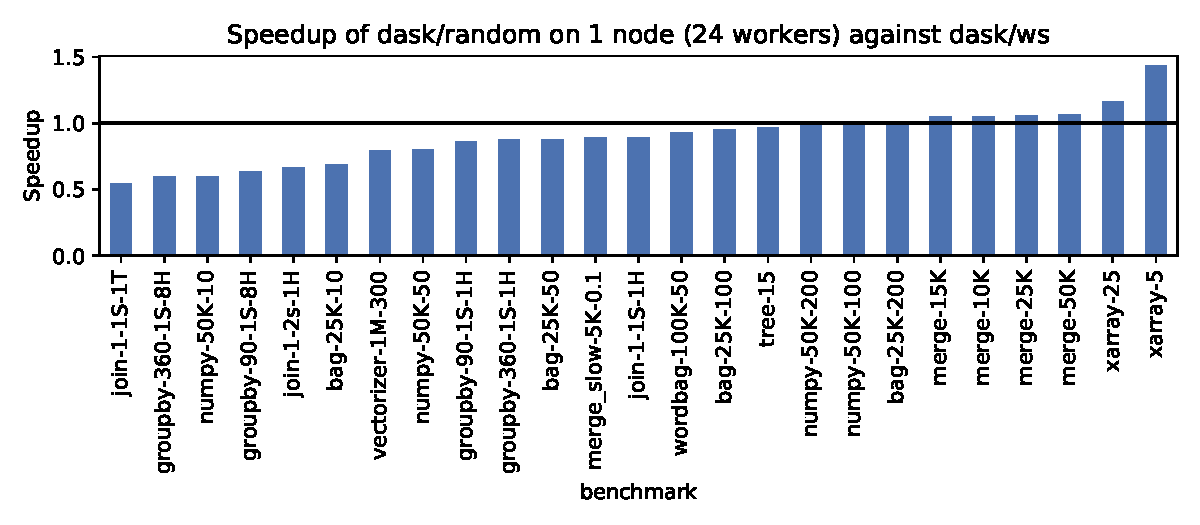
\includegraphics[width=0.9\textwidth]{imgs/rsds/charts/speedup-dask-random-1}
	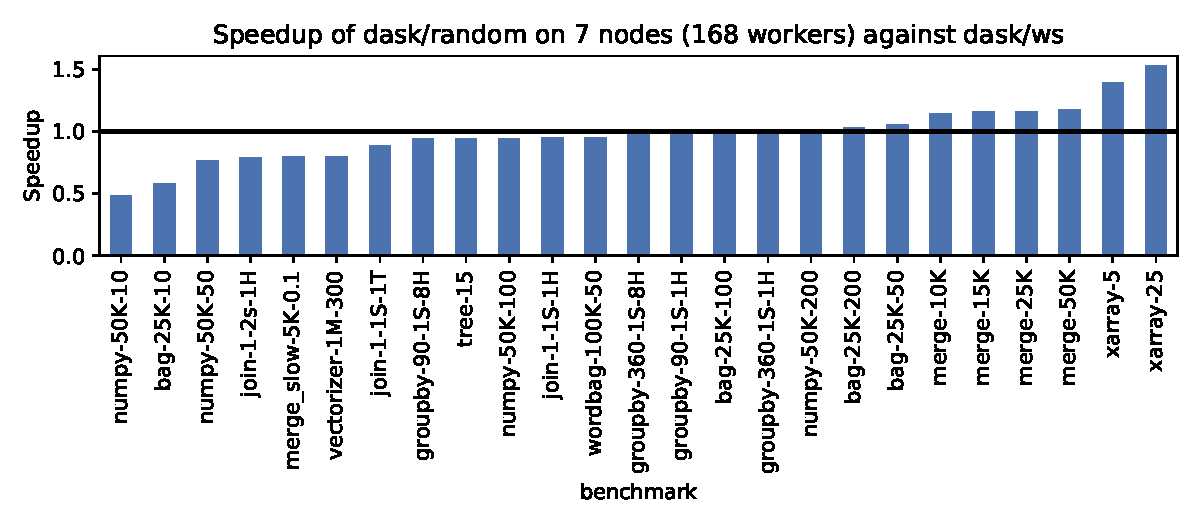
\includegraphics[width=0.9\textwidth]{imgs/rsds/charts/speedup-dask-random-7}
	\caption{Speedup of \dask{}/random scheduler; \dask{}/ws is baseline.}
	\label{fig:dask-ws-vs-random}
\end{figure}

We can observe the results of benchmarks that compare \dask{} using its baseline
work-stealing scheduler vs a completely random scheduler in Figure~\ref{fig:dask-ws-vs-random}. Based
on these results, it is clear that the random scheduler fares relatively well on both small and
medium sized clusters. At worst, it produces a twice longer makespan, but overall it is quite close
to the performance of the work-stealing scheduler, and in some cases it even outperforms it with a
$1.4\times$ speedup.

If we aggregate the results with a geometric mean, the random scheduler achieves
$88\%$ of the performance of the work-stealing scheduler with a single node, and
$95\%$ with seven nodes. The performance of the random scheduler thus gets closer
to the performance of work-stealing when more workers are used.

There are two effects that explain the reasonable performance of the random scheduler. Firstly, the
computational complexity of work-stealing scales with the number of available workers. With more
workers, the work-stealing scheduler has to perform more work to compute where should the tasks be
computed, and it also generates additional network traffic by sending task stealing messages
between workers. On the other hand, a random scheduler has a fixed computation cost per task,
completely independent of the worker count, as it simply chooses a worker randomly, and it also
sends no additional network messages other than one worker assignment per task. The difference in
computational overhead between these two schedulers will be examined in more detail in the
following experiment.

The second effect is also related to the fact that the random scheduler performs better with more
workers. Our benchmark set is compute-bound, so if there is a large enough number of workers
(relative to the number of tasks), it might not be that difficult for the scheduler to saturate all
the workers, even with a random schedule, as long as the task graph structure is not very
complicated. Furthermore, if the scheduler wants to utilize all computational power of a cluster
with many workers, network transfers are less avoidable, which decreases the chance that a random
scheduler induces an unnecessary data transfer that could have been avoided by a smarter scheduler.

The results of this experiment suggest that in certain scenarios, a complex scheduling algorithm is
not needed and a random schedule is sufficient for \dask{}. This shows that the
scheduler might not be its main bottleneck. We will also examine this in the following experiments.

\subsubsection*{Overhead per task}
We have seen that a random scheduler can be surprisingly competitive with the work-stealing
scheduling implementation in \dask{}. In this experiment, we will further examine
this effect by computing the inner overhead of \dask{} per each executed task. To
isolate the effect of the executed tasks, this experiment was performed using a modified version of
\dask{}, using a configuration that we call \emph{zero worker}. In this mode,
\dask{} workers essentially turn each task into an empty function that does not
perform any computation. This idealized worker implementation helps us to understand the
fundamental overhead of the \dask{} runtime, independent of the specific tasks that
are being executed. Note that even though all tasks in this mode are basically the same, the shape
and size of the benchmarked task graph are still important, since they affect the scheduler's
performance and also bookkeeping overhead of the runtime.

\begin{figure}
	\centering
	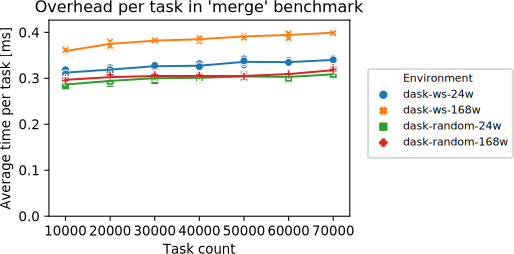
\includegraphics[width=0.5\textwidth]{imgs/rsds/charts/dask-merge-task-scaling}
	\caption{Overhead per task in \dask{} with an increasing number of tasks.}
	\label{fig:dask-merge-task-scaling}
\end{figure}

Using this special mode, we have evaluated the average runtime overhead per each task, which is
calculated as the total makespan divided by the number of tasks in the executed task graph.
Figure~\ref{fig:dask-merge-task-scaling} shows the average overhead per task for the \texttt{merge}
benchmark, we can see the average overhead per each task (the Y axis), and how it changes with an
increasing number of tasks (X axis). We can observe that the overhead of the random scheduler is
smaller the overhead of the work-stealing scheduler, as expected. We can also see that the overhead
per task increases with an increasing number of tasks, for both schedulers. There is also a
distinct increase of overhead between the overhead with $24$ workers (one node)
and $168$ workers (seven nodes) for the work-stealing scheduler.

\begin{figure}
	\centering
	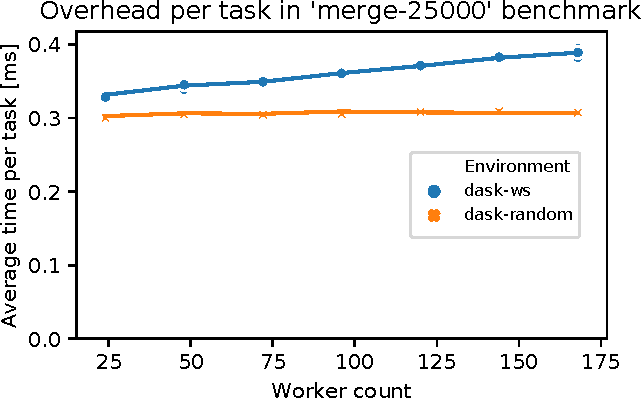
\includegraphics[width=0.5\textwidth]{imgs/rsds/charts/dask-merge-worker-scaling}
	\caption{Overhead per task in \dask{} with an increasing number of workers.}
	\label{fig:dask-merge-worker-scaling}
\end{figure}

This can be examined in more detail in Figure~\ref{fig:dask-merge-worker-scaling}, which shows how does the
overhead increase when more workers are available. It is clear that the performance of the
work-stealing degrades rapidly when more workers are added to the custer, while the overhead of th
random scheduler stays almost constant, inependent on the number of workers.

The \dask{} manual states that ``Each task suffers about 1ms of overhead. A small
computation and a network roundtrip can complete in less than 10ms.''~\footnote{\url{https://distributed.dask.org/en/latest}}. Our
experiment shows that the overhead is less than $1ms$ for most of our benchmarks.

\begin{figure}
	\centering
	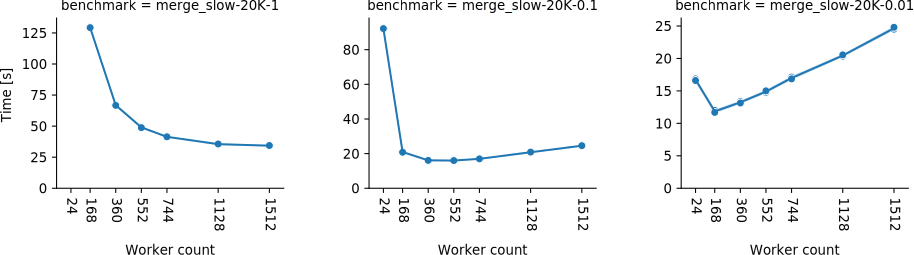
\includegraphics[width=0.9\textwidth]{imgs/rsds/charts/dask-strong-scaling}
	\caption{Strong scaling of \dask{} with different task durations ($1000ms$, $100ms$ and
		$10ms$).}
	\label{fig:dask-strong-scaling}
\end{figure}

The overhead per task is an important property of the task runtime, since it determines the minimal
duration of a task that is still viable for parallel execution with that runtime. If the duration
of a task is similar or smaller than the overhead of the runtime itself, executing such task with
the runtime will probably not yield any speedup. This is demonstrated in
Figure~\ref{fig:dask-strong-scaling}, which shows the strong scaling of \dask{} on the
$merge\_slow$ benchmark. The three charts demonstrate its scaling with tasks that take $1000ms$, $100ms$
and $10ms$ (respectively). With tasks that take a second, \dask{} is able to scale relatively
well up to $1512$ workers. However, when tasks take ten times less time, it only scales up to
around $360$ workers, and when tasks take only $10ms$, \dask{} scales to around $168$ workers,
and adding further workers makes the makespan longer.

The results of this experiment indicate that the general runtime overhead of \dask{} mainly
grows with an increasing number of tasks, no matter which scheduler is used. On the other hand, overhead
of the work-stealing scheduler grows primarily with the number of workers. They also show that
the minimum duration of tasks executed by \dask{} should be taken into account, to avoid
introducing too much runtime overhead.

These results also suggest that \dask{} can struggle with a larger number of workers. This
wouldn't be an issue on its own, as every task runtime will have its scaling limit. However, due
to the already mentioned effect of GIL, \dask{} users might be forced to use more workers than
would be otherwise necessary to achieve reasonable performance. We will examine this in the next
experiment.

\subsection*{The effect of GIL}

\begin{figure}
	\centering
	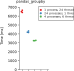
\includegraphics[width=0.3\linewidth]{./imgs/rsds/charts/dask-gil-scaling}
	\caption{Effect of GIL on the performance of \dask{}}
	\label{fig:dask-gil-scaling}
\end{figure}

Figure~\ref{fig:dask-gil-scaling} demonstrates the effect of the GIL

%TODO: conclusion - Dask doesn't scale well, needs tuning

%%%%%%%%%%%%%%%%%%%%%%%%%%%
%TODO: RSDS

\section{\rsds{} (alternative \dask{} server)}
\label{sec:rsds-description}

In order to measure how could \dask{}'s performance be improved if it had a more
efficient runtime, as a second main contribution of this work we have developed
\rsds{}, an open-source drop-in replacement for the \dask{} central
server\footnoteurl{https://github.com/it4innovations/rsds}. It was built from the ground up with a focus on runtime efficiency
and scheduler modularity, but at the same time we have designed it to be compatible with the
\dask{} protocol, so it could be used by existing \dask{} users to
speed up their task workflows.


\begin{figure}[tbph]
	\centering
	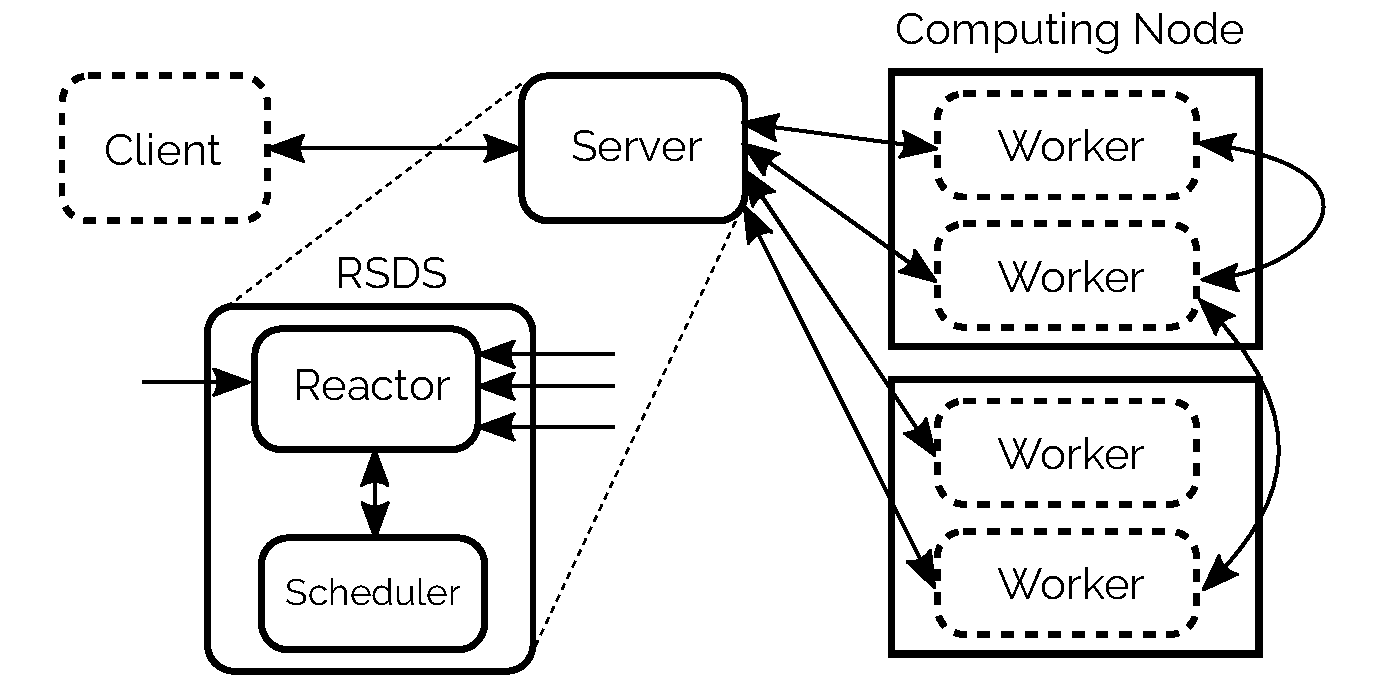
\includegraphics[width=0.8\linewidth]{./imgs/rsds/rsds-architecture}
	\caption{Architecture of \rsds{} (\dask{} components are dashed)}
	\label{fig:rsds-architecture}
\end{figure}

\section{Task runtime benchmarks}
\label{sec:rsds-dask-rsds-comparison}

\subsection*{Benchmark configuration}


TODO: chart from Works 2020 slides with Dask overhead scaling, and worker/thread configuration

----------------

- describe Dask
- describe benchmarks
- describe random scheduler performance

%EXPAND: compare RSDS vs Dask (overhead, scaling, zero-worker)

\section{Comparison of Dask and RSDS}
\label{sec:rsds-dask-comparison}

%%%%% TEZE %%%%%
%%%%% Analysis/Conclusion %%%%%
The scheduler is not the only part of a task runtime that can cause bottlenecks in task graph
execution. We have analysed an existing and quite popular task runtime
\dask{}~\cite{dask} in \emph{Runtime vs Scheduler: Analyzing Dask's Overheads}~\cite{rsds},
both to find out what bottlenecks does it have, and also to benchmark various scheduling algorithms
with \dask{}, to test them ``in the wild'' and thus better validate our results
from~\cite{estee}.

Our analysis has demonstrated that \dask{} was bottlenecked not so much by its
scheduler, but by the runtime (in)efficiency of its central server. The inefficiencies were caused
partly by the design of its communication protocol, but mainly by the fact that
\dask{} is implemented in Python, which makes it difficult to fully utilize the
available hardware potential. We have also found out that it was impractical to swap
\dask{}'s scheduler implementation for another one, since its built-in
work-stealing scheduling algorithm was quite firmly integrated into its components.

In order to measure how could \dask{}'s performance be improved if it had a more
efficient runtime, as a second main contribution of this work we have developed
\rsds{}, an open-source drop-in replacement for the \dask{} central
server\footnoteurl{https://github.com/it4innovations/rsds}. It was built from the ground up with a focus on runtime efficiency
and scheduler modularity, but at the same time we have designed it to be compatible with the
\dask{} protocol, so it could be used by existing \dask{} users to
speed up their task workflows.

We have performed a series of experiments where we have compared the performance of
\rsds{} vs \dask{}. Since \rsds{} allows its users
to plug in a different scheduling algorithm easily, we have also compared the performance of
\rsds{} with various scheduling algorithms. The experiments were conducted on task
graphs generated from tracing real-world \dask{} task workflows, to make sure that
we were benchmarking realistic use-cases.

The results of our experiments indicate that optimizing the runtime is definitely a worthy effort
to pursuit, as \rsds{} has been able to outperform \dask{} in
various scenarios, even though it used a much simpler work-stealing scheduling algorithm. We have
also been able to validate our results from~\cite{estee}, for example that even a random
scheduler is indeed competitive with other scheduling approaches in many scenarios.

We have contacted the authors and maintainers of \dask{} and discussed our
\rsds{} approach with
them\footnoteurl{https://github.com/dask/distributed/issues/3139}\footnoteurl{https://github .com/dask/distributed/issues/3783}\footnoteurl{https://github.com/dask/distributed/issues/3872}. Some of its ideas have
been adapted in the \dask{} project and led to improving its performance.

An interesting insight regarding task schedulers that we have gained from our work done
in~\cite{estee,rsds} is just how much important are the specific details of scheduling
algorithm implementations. While trying to implement various scheduling algorithms from existing
literature, we have realized that they are often incomplete. Details like how often should the
algorithm be invoked or how to choose between workers which receive an equal scheduling priority
from the algorithm are often left up to the implementor. However, our experiments have shown us
that these seemingly minor details can have a significant effect on the performance of the
scheduler, both in terms of runtime efficiency and the quality of its generated schedules.
